\documentclass[10pt]{article}
\usepackage[utf8]{inputenc}
%\usepackage[upright]{fourier}%withot fourier  symb = $\altersquare$
\usepackage{alterqcm}
\usepackage{fullpage,longtable}

\usepackage[a4paper,bindingoffset=0.2in,%
            left=0.75cm,right=2cm,top=2cm,bottom=1cm,%
            footskip=.25in]{geometry}
            
\usepackage{booktabs}

\usepackage{graphicx}
\usepackage{amsmath}
\usepackage{amssymb}
\usepackage{wrapfig}
\usepackage{tabularx,ragged2e,booktabs}
\usepackage{subfig}
\newcolumntype{C}[1]{>{\centering\arraybackslash}p{#1}}
\newcommand{\checked}{$\text{\rlap{$\checkmark$}}\square$}
\newcommand{\unchecked}{$\square$}
\newcommand{\qedsymbol}{$\blacksquare$}

\let\emptyset\varnothing

\begin{document}
\parindent0pt

Exam, 28 January, 2022. \\

For each of the 7 lectures there are 6 MCQ questions + 1 Open question, yielding $7 \times 7 = 49$ questions in total. There is one correct answer for each MCQ question. Mark the answer on the answer sheet (note the ordering of the A,B,C,D options). Closed book exam: No books, notes, phones, etc allowed. Good luck! 

\begin{flushright}

\begin{tabular}{|p{8cm}@{\hskip 0.5cm}p{10.5cm}|} 
\toprule  
\textbf{Question 1} & \emph{Lecture 1 \hfill Histograms and color}  \\ 
\midrule 
\begin{tabular}{p{8cm}}
From the RGB cube, the color plane defined by fixing the coordinate R to 1 (ie: R=1) looks like: 
\end{tabular} &
\begin{tabular}{p{10.5cm}}


\textbf{\unchecked A:} Green, Blue, White \newline 


\textbf{\unchecked B:} Red, Purple, Black \newline 


\textbf{\unchecked C:} Red, Yellow, White \newline 


\textbf{\unchecked D:} Yellow, Purple, Black \newline 


\textbf{\unchecked E:} Yellow, Red, Black \newline 


\textbf{\unchecked F:} Red, Blue, Black \newline 


\end{tabular} \\ \bottomrule
\end{tabular}

\begin{tabular}{|p{8cm}@{\hskip 0.5cm}p{10.5cm}|} 
\toprule  
\textbf{Question 2} & \emph{Lecture 1 \hfill Histograms and color}  \\ 
\midrule 
\begin{tabular}{p{8cm}}
Consider these color pairs: RGB(1, 0, 0)-HSI(0, 1, 1); RGB(1, 1, 1)-HSI(0, 0, 1); RGB(0, 0, 0)-HSI(0, 0, 1); RGB(0, 0, 1)-HSI(0, 1, 1/3). How many pairs represents the same color? 
\end{tabular} &
\begin{tabular}{p{10.5cm}}


\textbf{\unchecked A:} Only 1 pair \newline 


\textbf{\unchecked B:} 2 pairs \newline 


\textbf{\unchecked C:} 3 pairs \newline 


\end{tabular} \\ \bottomrule
\end{tabular}

\begin{tabular}{|p{8cm}@{\hskip 0.5cm}p{10.5cm}|} 
\toprule  
\textbf{Question 3} & \emph{Lecture 1 \hfill Histograms and color}  \\ 
\midrule 
\begin{tabular}{p{8cm}}
Using point processing on pixels with a typical 8-bit per channel RGB encoding, which operations do we need to apply to each channel to obtain an image with inverted colours? (x is the pixel from the input image) 
\end{tabular} &
\begin{tabular}{p{10.5cm}}


\textbf{\unchecked A:} Subtract 255 from x \newline 


\textbf{\unchecked B:} Multiply x by -1 and add (255*3) \newline 


\textbf{\unchecked C:} Multiply x by -1 and add 255 \newline 


\textbf{\unchecked D:} Subtract 128 from x \newline 


\end{tabular} \\ \bottomrule
\end{tabular}

\begin{tabular}{|p{19cm}|} 
\toprule  
\textbf{Question 4}\hfill \emph{Lecture 1 \hfill Histograms and color}  \\
\midrule 
Open question: For this 3x4 intensity image and its pixel values. \newline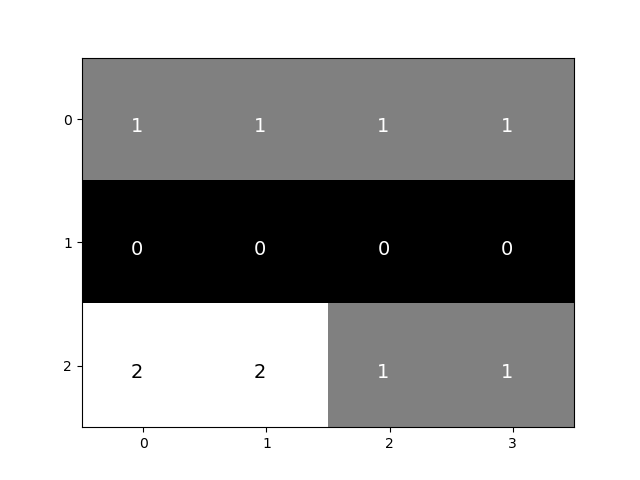
\includegraphics[width=7cm,height=6cm,keepaspectratio]{example.png} \newline\newline Draw its histogram and apply histogram equalization. Give all the performed steps. \\ 
\bottomrule
\end{tabular}


\end{flushright}

End of exam.
\end{document}  
